\documentclass{beamer}
\usepackage{amsmath,graphics}
\usepackage{amssymb}

\usetheme{default}
\usepackage{xcolor}

\definecolor{solarizedBase03}{HTML}{002B36}
\definecolor{solarizedBase02}{HTML}{073642}
\definecolor{solarizedBase01}{HTML}{586e75}
\definecolor{solarizedBase00}{HTML}{657b83}
\definecolor{solarizedBase0}{HTML}{839496}
\definecolor{solarizedBase1}{HTML}{93a1a1}
\definecolor{solarizedBase2}{HTML}{EEE8D5}
\definecolor{solarizedBase3}{HTML}{FDF6E3}
\definecolor{solarizedYellow}{HTML}{B58900}
\definecolor{solarizedOrange}{HTML}{CB4B16}
\definecolor{solarizedRed}{HTML}{DC322F}
\definecolor{solarizedMagenta}{HTML}{D33682}
\definecolor{solarizedViolet}{HTML}{6C71C4}
%\definecolor{solarizedBlue}{HTML}{268BD2}
\definecolor{solarizedBlue}{HTML}{134676}
\definecolor{solarizedCyan}{HTML}{2AA198}
\definecolor{solarizedGreen}{HTML}{859900}
\definecolor{myBlue}{HTML}{162DB0}%{261CA4}
\setbeamercolor*{item}{fg=myBlue}
\setbeamercolor{normal text}{fg=solarizedBase03, bg=solarizedBase3}
\setbeamercolor{alerted text}{fg=myBlue}
\setbeamercolor{example text}{fg=myBlue, bg=solarizedBase3}
\setbeamercolor*{frametitle}{fg=solarizedRed}
\setbeamercolor*{title}{fg=solarizedRed}
\setbeamercolor{block title}{fg=myBlue, bg=solarizedBase3}
\setbeameroption{hide notes}
\setbeamertemplate{note page}[plain]
\beamertemplatenavigationsymbolsempty
\usefonttheme{professionalfonts}
\usefonttheme{serif}

\usepackage{fourier}

\def\vec#1{\mathchoice{\mbox{\boldmath$\displaystyle#1$}}
{\mbox{\boldmath$\textstyle#1$}}
{\mbox{\boldmath$\scriptstyle#1$}}
{\mbox{\boldmath$\scriptscriptstyle#1$}}}
\definecolor{OwnGrey}{rgb}{0.560,0.000,0.000} % #999999
\definecolor{OwnBlue}{rgb}{0.121,0.398,0.711} % #1f64b0
\definecolor{red4}{rgb}{0.5,0,0}
\definecolor{blue4}{rgb}{0,0,0.5}
\definecolor{Blue}{rgb}{0,0,0.66}
\definecolor{LightBlue}{rgb}{0.9,0.9,1}
\definecolor{Green}{rgb}{0,0.5,0}
\definecolor{LightGreen}{rgb}{0.9,1,0.9}
\definecolor{Red}{rgb}{0.9,0,0}
\definecolor{LightRed}{rgb}{1,0.9,0.9}
\definecolor{White}{gray}{1}
\definecolor{Black}{gray}{0}
\definecolor{LightGray}{gray}{0.8}
\definecolor{Orange}{rgb}{0.1,0.2,1}
\setbeamerfont{sidebar right}{size=\scriptsize}
\setbeamercolor{sidebar right}{fg=Black}

\renewcommand{\emph}[1]{{\textcolor{solarizedRed}{\itshape #1}}}

\newcommand\dd{\mathrm d}
\newcommand\eul{\mathrm e}

\newcommand\cA{\mathcal A}
\newcommand\cB{\mathcal B}
\newcommand\cC{\mathcal C}
\newcommand\cD{\mathcal D}
\newcommand\cE{\mathcal E}
\newcommand\cF{\mathcal F}
\newcommand\cG{\mathcal G}
\newcommand\cH{\mathcal H}
\newcommand\cI{\mathcal I}
\newcommand\cJ{\mathcal J}
\newcommand\cK{\mathcal K}
\newcommand\cL{\mathcal L}
\newcommand\cM{\mathcal M}
\newcommand\cN{\mathcal N}
\newcommand\cO{\mathcal O}
\newcommand\cP{\mathcal P}
\newcommand\cQ{\mathcal Q}
\newcommand\cR{\mathcal R}
\newcommand\cS{\mathcal S}
\newcommand\cT{\mathcal T}
\newcommand\cU{\mathcal U}
\newcommand\cV{\mathcal V}
\newcommand\cW{\mathcal W}
\newcommand\cX{\mathcal X}
\newcommand\cY{\mathcal Y}
\newcommand\cZ{\mathcal Z}

\newcommand\fA{\mathfrak A}
\newcommand\fB{\mathfrak B}
\newcommand\fC{\mathfrak C}
\newcommand\fD{\mathfrak D}
\newcommand\fE{\mathfrak E}
\newcommand\fF{\mathfrak F}
\newcommand\fG{\mathfrak G}
\newcommand\fH{\mathfrak H}
\newcommand\fI{\mathfrak I}
\newcommand\fJ{\mathfrak J}
\newcommand\fK{\mathfrak K}
\newcommand\fL{\mathfrak L}
\newcommand\fM{\mathfrak M}
\newcommand\fN{\mathfrak N}
\newcommand\fO{\mathfrak O}
\newcommand\fP{\mathfrak P}
\newcommand\fQ{\mathfrak Q}
\newcommand\fR{\mathfrak R}
\newcommand\fS{\mathfrak S}
\newcommand\fT{\mathfrak T}
\newcommand\fU{\mathfrak U}
\newcommand\fV{\mathfrak V}
\newcommand\fW{\mathfrak W}
\newcommand\fX{\mathfrak X}
\newcommand\fY{\mathfrak Y}
\newcommand\fZ{\mathfrak Z}

\newcommand\fa{\mathfrak a}
\newcommand\fb{\mathfrak b}
\newcommand\fc{\mathfrak c}
\newcommand\fd{\mathfrak d}
\newcommand\fe{\mathfrak e}
\newcommand\ff{\mathfrak f}
\newcommand\fg{\mathfrak g}
\newcommand\fh{\mathfrak h}
%\newcommand\fi{\mathfrak i}
\newcommand\fj{\mathfrak j}
\newcommand\fk{\mathfrak k}
\newcommand\fl{\mathfrak l}
\newcommand\fm{\mathfrak m}
\newcommand\fn{\mathfrak n}
\newcommand\fo{\mathfrak o}
\newcommand\fp{\mathfrak p}
\newcommand\fq{\mathfrak q}
\newcommand\fr{\mathfrak r}
\newcommand\fs{\mathfrak s}
\newcommand\ft{\mathfrak t}
\newcommand\fu{\mathfrak u}
\newcommand\fv{\mathfrak v}
\newcommand\fw{\mathfrak w}
\newcommand\fx{\mathfrak x}
\newcommand\fy{\mathfrak y}
\newcommand\fz{\mathfrak z}

\newcommand\vA{\vec A}
\newcommand\vB{\vec B}
\newcommand\vC{\vec C}
\newcommand\vD{\vec D}
\newcommand\vE{\vec E}
\newcommand\vF{\vec F}
\newcommand\vG{\vec G}
\newcommand\vH{\vec H}
\newcommand\vI{\vec I}
\newcommand\vJ{\vec J}
\newcommand\vK{\vec K}
\newcommand\vL{\vec L}
\newcommand\vM{\vec M}
\newcommand\vN{\vec N}
\newcommand\vO{\vec O}
\newcommand\vP{\vec P}
\newcommand\vQ{\vec Q}
\newcommand\vR{\vec R}
\newcommand\vS{\vec S}
\newcommand\vT{\vec T}
\newcommand\vU{\vec U}
\newcommand\vV{\vec V}
\newcommand\vW{\vec W}
\newcommand\vX{\vec X}
\newcommand\vY{\vec Y}
\newcommand\vZ{\vec Z}

\newcommand\va{\vec a}
\newcommand\vb{\vec b}
\newcommand\vc{\vec c}
\newcommand\vd{\vec d}
\newcommand\ve{\vec e}
\newcommand\vf{\vec f}
\newcommand\vg{\vec g}
\newcommand\vh{\vec h}
\newcommand\vi{\vec i}
\newcommand\vj{\vec j}
\newcommand\vk{\vec k}
\newcommand\vl{\vec l}
\newcommand\vm{\vec m}
\newcommand\vn{\vec n}
\newcommand\vo{\vec o}
\newcommand\vp{\vec p}
\newcommand\vq{\vec q}
\newcommand\vr{\vec r}
\newcommand\vs{\vec s}
\newcommand\vt{\vec t}
\newcommand\vu{\vec u}
\newcommand\vv{\vec v}
\newcommand\vw{\vec w}
\newcommand\vx{\vec x}
\newcommand\vy{\vec y}
\newcommand\vz{\vec z}

\renewcommand\AA{\mathbb A}
\newcommand\NN{\mathbb N}
\newcommand\ZZ{\mathbb Z}
\newcommand\PP{\mathbb P}
\newcommand\QQ{\mathbb Q}
\newcommand\RR{\mathbb R}
\newcommand\RRpos{\mathbb R_{\geq0}}
\renewcommand\SS{\mathbb S}
\newcommand\CC{\mathbb C}

\newcommand{\ord}{\mathrm{ord}}
\newcommand{\id}{\mathrm{id}}
\newcommand{\pr}{\mathrm{P}}
\newcommand{\Vol}{\mathrm{vol}}
\newcommand\norm[1]{\left\|{#1}\right\|} 
\newcommand\sign{\mathrm{sign}}
\newcommand{\eps}{\varepsilon}
\newcommand{\abs}[1]{\left|#1\right|}
\newcommand\bc[1]{\left({#1}\right)} 
\newcommand\cbc[1]{\left\{{#1}\right\}} 
\newcommand\bcfr[2]{\bc{\frac{#1}{#2}}} 
\newcommand{\bck}[1]{\left\langle{#1}\right\rangle} 
\newcommand\brk[1]{\left\lbrack{#1}\right\rbrack} 
\newcommand\scal[2]{\bck{{#1},{#2}}} 
\newcommand{\vecone}{\mathbb{1}}
\newcommand{\tensor}{\otimes}
\newcommand{\diag}{\mathrm{diag}}
\newcommand{\ggt}{\mathrm{ggT}}
\newcommand{\kgv}{\mathrm{kgV}}
\newcommand{\trans}{\top}

\newcommand{\Karonski}{Karo\'nski}
\newcommand{\Erdos}{Erd\H{o}s}
\newcommand{\Renyi}{R\'enyi}
\newcommand{\Lovasz}{Lov\'asz}
\newcommand{\Juhasz}{Juh\'asz}
\newcommand{\Bollobas}{Bollob\'as}
\newcommand{\Furedi}{F\"uredi}
\newcommand{\Komlos}{Koml\'os}
\newcommand{\Luczak}{\L uczak}
\newcommand{\Kucera}{Ku\v{c}era}
\newcommand{\Szemeredi}{Szemer\'edi}

\renewcommand{\ae}{\"a}
\renewcommand{\oe}{\"o}
\newcommand{\ue}{\"u}
\newcommand{\Ae}{\"A}
\newcommand{\Oe}{\"O}
\newcommand{\Ue}{\"U}

\newcommand{\im}{\mathrm{im}}
\newcommand{\rrk}{\mathrm{zrg}}
\newcommand{\crk}{\mathrm{srg}}
\newcommand{\rk}{\mathrm{rg}}
\newcommand{\GL}{\mathrm{GL}}
\newcommand{\SL}{\mathrm{SL}}
\newcommand{\SO}{\mathrm{SO}}
\newcommand{\nul}{\mathrm{nul}}
\newcommand{\eig}{\mathrm{eig}}

\newcommand{\mytitle}{Exponentialfunktion und Logarithmus}

\title[Annuma]{\mytitle}
\author[Amin Coja-Oghlan]{Amin Coja-Oghlan}
\institute[Frankfurt]{JWGUFFM}
\date{}

\begin{document}

\frame[plain]{\titlepage}

\begin{frame}\frametitle{\mytitle}
	\begin{block}{Worum geht es?}
		\begin{itemize}
			\item Wir haben Werkzeuge zur Analyse von Funktionen kennengelernt.
			\item Bisher kennen wir mit Ausnahme von Polynomen aber kaum Funktionen.
			\item Wir lernen nun zwei wichtige Funktionen kennen: Logarithmus und Exponentialfunktion.
		\end{itemize}
	\end{block}
\end{frame}

\begin{frame}\frametitle{\mytitle}
	\begin{block}{Definition}
			Der \emph{nat\ue rliche Logarithmus} ist die Funktion
				\begin{align*}
					\ln:(0,\infty)\to\RR,\qquad z\mapsto\int_1^z\frac{1}{x}\dd x.
				\end{align*}
	\end{block}
	{\itshape Weil die Funktion $x\mapsto\frac{1}{x}$ stetig ist, macht die Definition Sinn. Wer verwenden also das Integral, um eine neue Funktion zu definieren!}
\end{frame}

\begin{frame}\frametitle{\mytitle}
	\hfill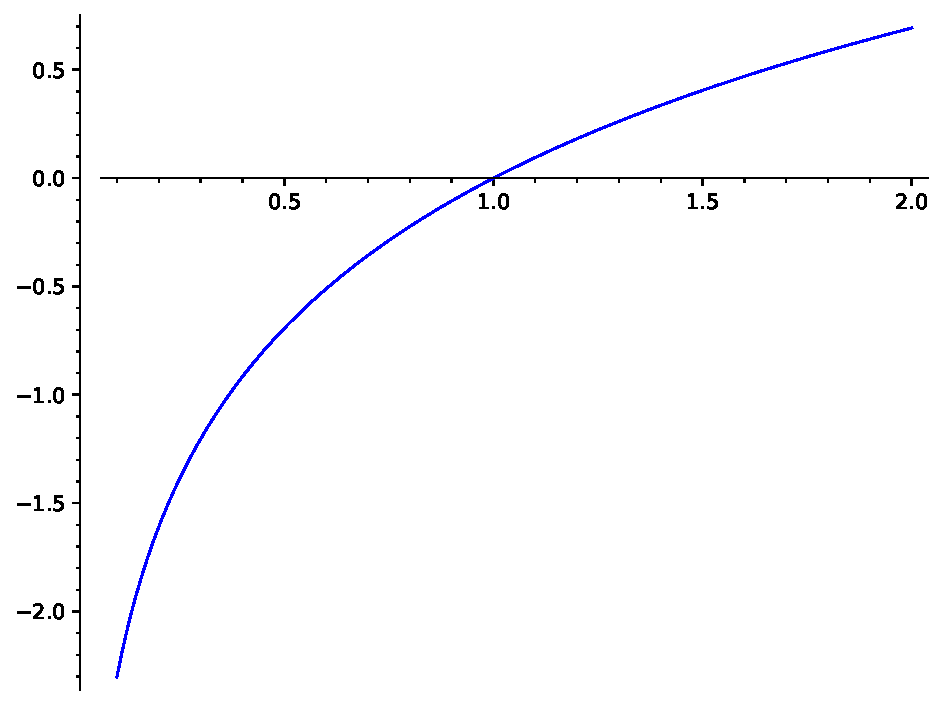
\includegraphics[height=30mm]{pics/plot_ln.pdf}
	\begin{block}{Eigenschaften des Logarithmus'}
	\begin{itemize}
		\item Es gilt $\ln(1)=0$, weil $\int_1^1\frac{\dd x}{x}=0$.
		\item Der Hauptsatz zeigt ferner, da\ss
			\begin{align*}
				\ln'(z)=\frac{1}{z}\qquad\mbox{f\ue r }z>0.
			\end{align*}
		\item Weil $1/z>0$ f\ue r $z>0$, ist der Logarithmus streng monoton wachsend.
	\end{itemize}
	\end{block}
\end{frame}

\begin{frame}\frametitle{\mytitle}
	\begin{block}{Lemma}
		F\ue r alle $a,b>0$ gilt $\ln(a\cdot b)=\ln(a)+\ln(b)$.
	\end{block}
	\begin{block}{Beweis}
	\begin{itemize}
	\item Wir betrachten die Funktionen
		\begin{align*}
			f:a\mapsto\ln(a\cdot b)\qquad g:a\mapsto\ln(a)+\ln(b).
		\end{align*}
	\item Offenbar gilt $f(1)=g(1)=\ln(b)$.
	\item Ferner erhalten wir $f'(a)=\frac{b}{a\cdot b}=\frac{1}{a}=g'(a).$
	\item Aus dem Hauptsatz folgt also
		\begin{align*}
			\ln(ab)&=f(a)=\int_1^af'(x)\dd x+f(1)\\&=\int_1^ag'(x)\dd x+g(1)=g(a)=\ln(a)+\ln(b).
		\end{align*}
	\end{itemize}
	\end{block}
\end{frame}

\begin{frame}\frametitle{\mytitle}
	\begin{block}{Weitere Eigenschaften}
		Sei $a>0$.
	\begin{itemize}
		\item Es gilt $\ln(1/a)=-\ln(a)$.
		\item F\ue r jede nat\ue rliche Zahl $n$ gilt $\ln(a^n)=n\ln(a)$.
		\item F\ue r jede rationale Zahl $q$ gilt $\ln(a^q)=q\ln(a)$.
		\item Die Funktion $\ln:(0,\infty)\to\RR$ ist also bijektiv.
	\end{itemize}
	\end{block}
\end{frame}

\begin{frame}\frametitle{\mytitle}
	\begin{block}{Definition}
		Die Umkehrfunktion der Funktion $\ln:(0,\infty)\to\RR$ hei\ss t die \emph{Exponentialfunktion}
		\begin{align*}
			\exp:\RR\to(0,\infty),\qquad z\mapsto\exp(z).
		\end{align*}
	\end{block}
\end{frame}

\begin{frame}\frametitle{\mytitle}
	\hfill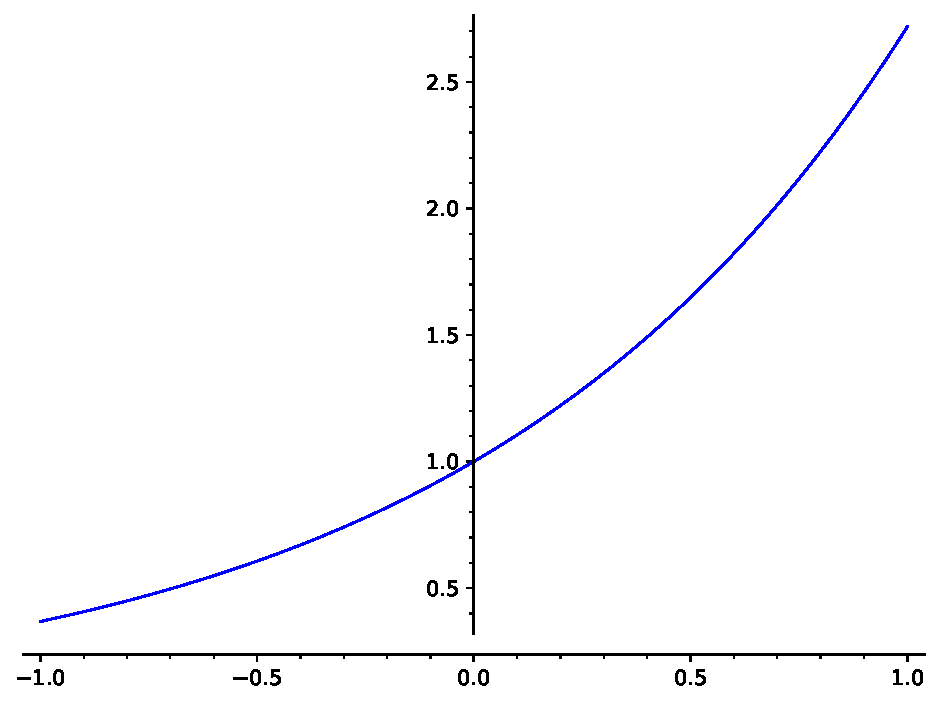
\includegraphics[height=30mm]{pics/plot_exp.pdf}
	\begin{block}{Eigenschaften der Exponentialfunktion}
	\begin{itemize}
	\item Die Exponentialfunktion ist streng monoton wachsend und bijektiv.
	\item Es gilt $\exp(0)=1$.
	\item Es gilt $\exp(a+b)=\exp(a)\cdot\exp(b)$.
	\item Der Satz \ue ber die Umkehrfunktion zeigt
		\begin{align*}
			\exp'(z)=\exp(z).
		\end{align*}
	\end{itemize}
	\end{block}
\end{frame}

\begin{frame}\frametitle{\mytitle}
	\begin{block}{Die allgemeine Potenz}
		Sei $x>0$.
	\begin{itemize}
		\item Aus der Schule kennen Sie die Potenzen $x^n$ f\ue r nat\ue rliche Exponenten $n\in\NN$:
			\begin{align*}
				x^n=\underbrace{x\cdot\enspace\cdots\enspace x}_{\mbox{$n$ mal}}.
			\end{align*}
		\item Wir verwenden ferner die Konvention $x^0=1$.
		\item Aus\ss erdem haben Sie $x^{1/n}$ kennengelernt als die positive L\oe sung $y$ der Gleichung
			\begin{align*}
			y^n=x,
			\end{align*}
			auch bekannt als die \alert{$n$-te Wurzel $\sqrt[n]x$ aus $x$}.
		\item Dar\ue ber hinaus kennen Sie die Schreibweise $x^{-1}=1/x$.
	\end{itemize}
	\end{block}
\end{frame}

\begin{frame}\frametitle{\mytitle}
	\begin{block}{Die allgemeine Potenz (fortgesetzt)}
	\begin{itemize}
		\item Daraus kann man die Potenzen $x^q$ f\ue r rationale Zahlen $\pm\frac{a}{b}$ ``zusammenreimen''.
		\item Dazu bestimmen wir zun\ae chst $y=x^{1/b}$, also die $b$-te Wurzel aus $x$.
		\item Diese erheben wir zur $a$-ten Potenz $x^{a/b}=y^a$.
		\item Wenn $q$ negativ ist, bilden wir schlie\ss lich $1/x^{a/b}$.
	\end{itemize}
	\end{block}
\end{frame}

\begin{frame}\frametitle{\mytitle}
	\begin{block}{Die allgemeine Potenz (fortgesetzt)}
	\begin{itemize}
		\item Auf diesem ``algebraischen'' Weg k\oe nnen wir jedoch nicht allgemeine reelle Potenzen definieren wie etwa
			\begin{align*}
				7^{\pi}.
			\end{align*}
		\item Um diese allgemeinen Potenzen einzuf\ue hren, verwenden wir die den Logarithmus und die Exponentialfunktion.
		\item Mit Hilfe von Logarithmus und Exponentialfunktion k\oe nnen wir schreiben
			\begin{align*}
				x^q=\exp(q\ln(x))\qquad\mbox{f\ue r }q\in\QQ.
			\end{align*}
		\item Nichts spricht dagegen, beliebige reelle Zahlen einzusetzen:
\begin{align*}
				x^r=\exp(r\ln(x))\qquad\mbox{f\ue r }r\in\RR.
			\end{align*}
	\end{itemize}
	\end{block}
\end{frame}

\begin{frame}\frametitle{\mytitle}
	\begin{block}{Ableitung und Integral allgemeiner Potenzen}
	\begin{itemize}
		\item F\ue r jeden Exponenten $r\in\RR$ erhalten wir die Ableitung
			\begin{align*}
				(x^r)'&=rx^{r-1}.
			\end{align*}
		\item Entsprechend gilt f\ue r Exponenten $r\neq-1$ die Formel
			\begin{align*}
				\int x^r\dd x&=\frac{x^{r+1}}{r+1}.
			\end{align*}
		\item \itshape Was ist mit $r=-1$?
	\end{itemize}
	\end{block}
\end{frame}

\begin{frame}\frametitle{\mytitle}
	\begin{block}{Die Eulerzahl}
	\begin{itemize}
		\item Wir definieren die \emph{Eulerzahl} als
			\begin{align*}
				\eul=\exp(1)=2.718281828459\cdots.
			\end{align*}
		\item Auf dem Weg \ue ber die allegemeine Potenz k\oe nnen wir dann die Exponentialfunktion schreiben als
			\begin{align*}
				\exp(x)=\eul^x\qquad(x\in\RR).
			\end{align*}
		\item Es gilt $\ln(\eul)=1$.
	\end{itemize}
	\end{block}
\end{frame}

\begin{frame}\frametitle{\mytitle}
	\begin{block}{Logarithmen mit allgemeinen Basen}
	\begin{itemize}
		\item Zu $b>1$ definieren wir den \emph{Logarithmus zur Basis $b$} als
			\begin{align*}
				\log_b:(0,\infty)\to\RR,\qquad z\mapsto\frac{\ln(z)}{\ln(b)}.
			\end{align*}
		\item Dieser hat die Eigenschaft
			\begin{align*}
				b^{\log_b z}&=z\qquad(z>0).
			\end{align*}
		\item Der nat\ue rliche Logarithmus ist derjenige zur Basis $\eul$, d.h.\
			\begin{align*}
				\ln(z)=\log_\eul(z).
			\end{align*}
	\end{itemize}
	\end{block}
\end{frame}

\begin{frame}\frametitle{\mytitle}
	\begin{block}{Exponentielles Wachstum}
	\begin{itemize}
		\item Angenommen $f:\RR\to\RR$ ist differenzierbar, so da\ss
			\begin{align*}
				f'(z)=a\cdot f(z)\qquad(a\in\RR).
			\end{align*}
		\item Dann gilt
			\begin{align*}
				f(z)=f(0)\cdot\exp(a z).
			\end{align*}
		\item Die Funktion $f$ ist also vollst\ae ndig durch ihre ``Wachstumsrate'' $a$ und durch den Startwert $f(0)$ bestimmt.
	\end{itemize}
	\end{block}
\end{frame}

\begin{frame}\frametitle{\mytitle}
	\begin{block}{Zusammenfassung}
	\begin{itemize}
		\item Wir haben den Logarithmus und die Exponentialfunktion kennengelernt.
		\item Diese Erm\oe glichen die Definition allgemeiner reeller Potenzen.
	\end{itemize}
	\end{block}
\end{frame}
\end{document}
